% ch16b Electrons at strong coupling: Mottness, part b (书页 380-399 / 分册p028-047)
%--TAIL--
\begin{figure}[H]\centering
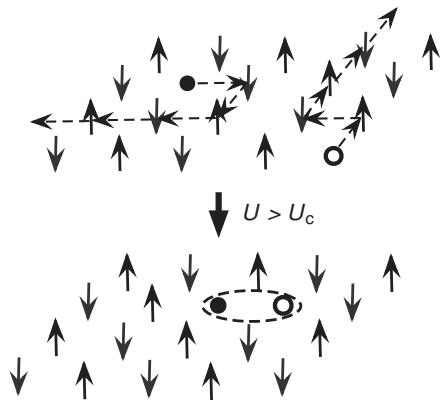
\includegraphics[width=0.52\textwidth]{figs/ch16/fig_16.7.jpg}
\caption*{图 16.7\quad 莫特提出的母体材料（半填充能带）中绝缘态的机制。上（下）箭头表示自旋向上（向下）的电子。当在位相互作用 $U$ 低于临界值时，双占据格点（实心圆点）与空穴（空心圆圈）可以自由输运；当 $U$ 高于临界值时，它们被束缚成局域的对，从而无法导电。}\label{fig:auto:16.7}
\end{figure}

通常都被丢弃。然而我们看到，若对算符作变换，它们便会自然出现，并贡献出与自旋交换项同阶的 $t^{2}/U$ 项。因此，把它们排除在外并没有什么系统性的依据。

\section{动力学谱权重转移}

微扰分析清楚表明，莫特绝缘态并不像原子极限图像让我们相信的那样容易理解。问题在于，双占据显式地出现在基态之中。因此，莫特能隙不能简单地看成到第一个含双占据的态之间的能隙。尽管如此，电荷能隙的判据仍然可以严格表述。如图 16.7 所描绘，双占据会留下一个空格点。这个空格点也许不必再激发到上能带就能自由移动。若果真如此，半填充能带实际上是导体。莫特（[M1949]）在其经典论文中指出了这一点，并论证：要使半填充能带绝缘，空格点与双占据格点之间必须存在某种束缚（见图 16.7）。事实上，此后若干研究者，例如 Kohn（[K1964]）、Fulde（[KHF1982]）以及 Castellani 及其合作者（[C1979]），都指出莫特绝缘体可以看成这样一种态：其中双占据是局域化的，而在导电态中则是退局域化的。因此，莫特转变到局域化状态时所涉及的自由度，并不显式地包含在初始的高能量紫外（UV）完备模型之中。也就是说，莫特能隙是动力学产生的，任何针对莫特体系的单电子描述都是无效的。虽然有序化可以直接从哈伯德模型的弱耦合或强耦合（$t/U$）分析中得到理解，束缚态的形成却不能，因为它从根本上源于基本场的重组。

\begin{figure}[H]\centering
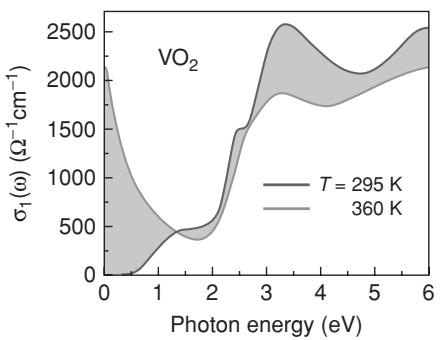
\includegraphics[width=0.48\textwidth]{figs/ch16/fig_16.8_a.jpg}\hfill
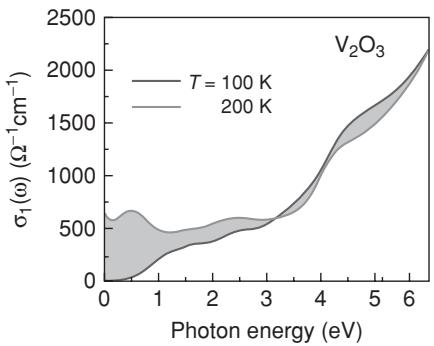
\includegraphics[width=0.48\textwidth]{figs/ch16/fig_16.8_b.jpg}
\caption*{图 16.8\quad $\mathrm{VO}_2$ 与 $\mathrm{V}_2\mathrm{O}_3$ 在莫特绝缘态开始出现的温度之上、之下的光电导（optical conductivity）实部。在 $\mathrm{VO}_2$ 和 $\mathrm{V}_2\mathrm{O}_3$ 中，向绝缘态的转变都伴随着谱权重从化学势附近向远至 6 eV 处的态的转移。这种向莫特态转变时谱权重的大规模重组是莫特转变的普遍特征。数据翻印自 Qazilbash 等，Phys. Rev. B 77, 115121 (2008)。}\label{fig:auto:16.8}
\end{figure}

它标志着微扰论的失效，正如我们在近藤问题中已经看到的那样——低温下的自由度是初始哈密顿量中并不存在的束缚态。

正如上一节所见，莫特绝缘体的特征是单粒子电子格林函数沿动量空间中一个连通曲面消失。格林函数实部消失的一个前提是谱函数在化学势上下都必须非零。金属中，谱权重位于化学势附近。于是问题来了：能隙一旦打开，原本处于化学势处的谱权重到哪里去了？它是像平均场理论中那样被推到恰在能隙之上的态，还是在远远超过能隙的能量处重新出现？这个问题的答案直指莫特问题的核心。考虑经典的莫特体系 $\mathrm{VO}_2$，它在 340 K 以下转变为绝缘态。在该体系中，每个钒离子的价为 $+4$，给出半填充的 $d^{1}$ 组态。$\mathrm{VO}_2$ 的特别之处在于，它直到最低温度都不发生磁有序。然而，伴随而来的结构重排使强关联的作用变得模糊。随温度降低跨过转变时，结构从高度对称的四方金红石结构变为单斜结构，其中钒原子发生二聚化并相对 $c$ 轴倾转。此外，载流子密度（[G1971]）从高温下的 $10^{23}\,\mathrm{cm}^{-3}$ 降到低温下的 $10^{18}\,\mathrm{cm}^{-3}$。结果，$\mathrm{VO}_2$ 中出现了与大多数半填充能带同样的问题：绝缘态究竟来自对称性破缺，还是如图 16.7 所示的那样完全来自强关联？尽管莫特（[ZM1975; RLP1994]）指出 0.6 eV 的能隙——即 $\mathrm{VO}_2$ 的电荷能隙——超出了钒离子二聚化可能涉及的任何能量尺度，这个问题依然存在。用椭偏法（ellipsometry）探测的该体系的光学响应，在这里对裁决这一问题特别有用。图 16.8 所示的关键特征是：把温度降到 295 K（[Q2008]）——这一能量尺度远小于 0.6 eV——会导致谱权重从化学势附近的态（浅色线）转移到能量高得多的态（深色线），距离约 6 eV 甚至更远。谱权重重新分布所涉及的这些能量尺度远远超过与二聚化相关的尺度；但它们与 $U$ 尺度上的关联物理一致。这就是 Mott 性（Mottness），而且正如我们将看到的，即使转变到超导态，它依然存在。事实上，这种情形甚至在半填充能带中也出现，例如 $\mathrm{V}_2\mathrm{O}_3$，已知（[Q2008]）其绝缘态具有反铁磁有序。图 16.8 的第二个面板给出了 $\mathrm{V}_2\mathrm{O}_3$ 中金属—绝缘体转变时的类似光电导。与 $\mathrm{VO}_2$ 一样，向绝缘态的转变同样涉及谱权重从化学势向至少 6 eV 之外的态的转移。这种高、低能量尺度的混合是莫特体系中的普遍现象。因此，对电荷能隙而言，核心是携带着 $U$ 尺度的传播自由度，而不仅仅是与可能发生的某种有序现象相联系的较小的能量尺度。$\mathrm{VO}_2$ 中另一处奇特之处是，能隙打开的温度远小于能隙本身。事实上，$\mathrm{VO}_2$ 的 $\Delta/T_{\mathrm{MI}}\approx 20$，至少是 BCS 理论中相应比值的 10 倍。

\subsection{掺杂莫特绝缘体：铜氧面}

高温铜氧化物超导体代表了另一类莫特体系，它们表现出以 $\mathrm{VO}_2$ 为典型的同一种紫外—红外（UV--IR）混合。铜氧化物是层状钙钛矿，其活跃层为铜氧面，其电子结构如图 16.9(a) 所示。在与铜氧化物相关的四面体晶体场中，一个未配对电子位于 $d_{x^{2}-y^{2}}$ 轨道上。因此，只考虑哈伯德型的单带模型似乎是很自然的。然而，未掺杂的铜氧化物实际上是如图 16.9(b) 那样的电荷转移绝缘体（charge-transfer insulator）。在这类体系中，每个单胞内不止一个原子，此处是一个氧原子。$d_{x^{2}-y^{2}}$ 轨道与氧的 $p_{x}$、$p_{y}$ 轨道杂化，因而三带模型才是自然的。不过，只要在位排斥能 $U$ 是最大的能量尺度，且单胞内原子之间的杂化足够可观（[ZR1988; MES1993]），约化为单带哈伯德模型就是合理的。铜氧化物正是这种情形。因此，铜氧化物超导电性的秘密至少蕴含在二维哈伯德模型的解中。图 16.10 给出了 $\mathrm{YBa}_2\mathrm{Cu}_3\mathrm{O}_y$ 沿 $\mathrm{CuO}_2$ 面、氧掺杂量分别为 $y=6.1$ 和 $y=6.6$ 时的光电导（[C1990; L2005]）。在很好的近似下，$y=6.1$ 代表母体材料，其频率低于 1.2 eV（铜氧化物的光学能隙）的光吸收受到明显抑制。这与母体绝缘材料中的莫特能隙一致。而在掺杂体系 $y=6.6$ 中，低于 $\approx 1.2\,\mathrm{eV}$ 的光电导强抑制消失了，并伴随高能区（距化学势约 3 eV）谱强度的减小。这种行为类似于 $\mathrm{VO}_2$ 在 340 K 以上向金属态转变时谱权重的反转。事实上，这两个体系中，掺杂诱导的金属态与温度诱导的转变所涉及的能量尺度完全相同。这种发生在 $O(U)$ 能量尺度上的重组只能源于强的电子关联。

\begin{figure}[H]\centering
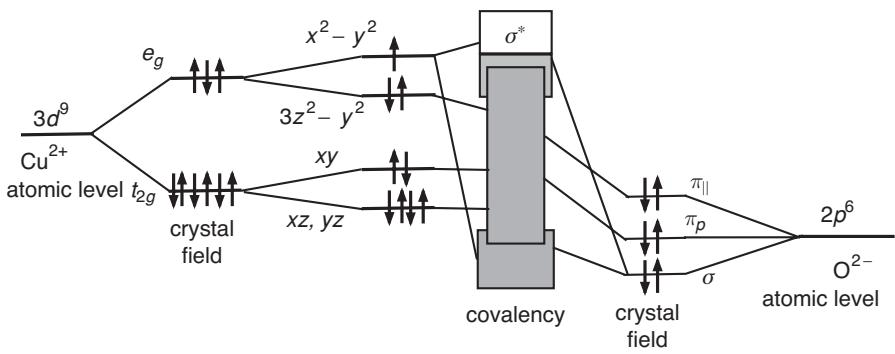
\includegraphics[width=0.8\textwidth]{figs/ch16/fig_16.9_a.jpg}

\vspace{0.5em}
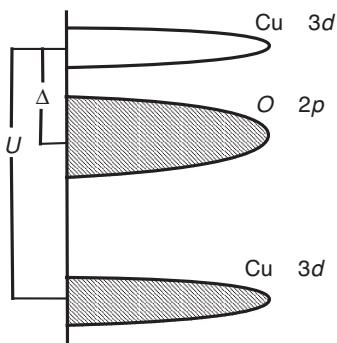
\includegraphics[width=0.42\textwidth]{figs/ch16/fig_16.9_b.jpg}
\caption*{图 16.9\quad 铜氧化物超导体中铜氧面的电子结构。(a) 铜氧面中原子的轨道占据与能级劈裂。上 $d$ 能级为单占据，但材料却是绝缘体，这使关联成为电子性质的主角。(b) 母体材料能带填充的示意描绘。$U$ 是两个电子占据 $\mathrm{d}_{x^{2}-y^{2}}$ 能级时的在位排斥能，$\Delta$ 是氧 $p$ 带与空的 $d$ 能级之间的能隙。在 $U\gg\Delta$ 且杂化足够大的极限下，电荷转移绝缘体可约化为单带哈伯德模型，从而等价于莫特绝缘体。}\label{fig:auto:16.9}
\end{figure}

光电导的探针是电流，因此它应当直接给出载流子总数的指示。正如本章开头所见，引入能带绝缘体或半导体的每个空穴都会在化学势上方产生一个准粒子。那么，在掺杂莫特绝缘体中会发生什么？我们猜想，由于谱权重从谱的高能部分转移过来，准粒子的数目必定超过裸掺杂量。事实正是如此。对光电导作积分，我们可以算出有效载流子数，或更准确地说是归一化载流子密度，
\begin{equation*}
N_{\mathrm{eff}}(\Omega)=\frac{2mV_{\mathrm{cell}}}{\pi e^{2}}\int_{0}^{\Omega}\sigma(\omega)\,\mathrm{d}\omega,\tag{16.116}
\end{equation*}
\begin{figure}[H]\centering
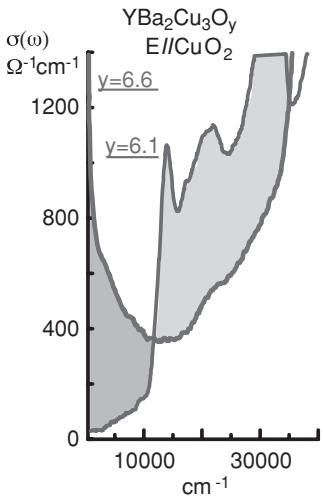
\includegraphics[width=0.32\textwidth]{figs/ch16/fig_16.10.jpg}
\caption*{图 16.10\quad $\mathrm{YBa}_2\mathrm{Cu}_3\mathrm{O}_y$（YBCO）在两个掺杂量下面内光电导的演化。在很好的近似下，$y=6.1$ 代表母体材料，$y=6.6$ 代表过掺杂样品。关键特征是：“母体”材料中 1.2 eV 以上的谱权重在掺杂后转移到化学势附近的态。翻印自 Cooper 等，Phys. Rev. B 47, 8233 (1993)。}\label{fig:auto:16.10}
\end{figure}
\begin{figure}[H]\centering
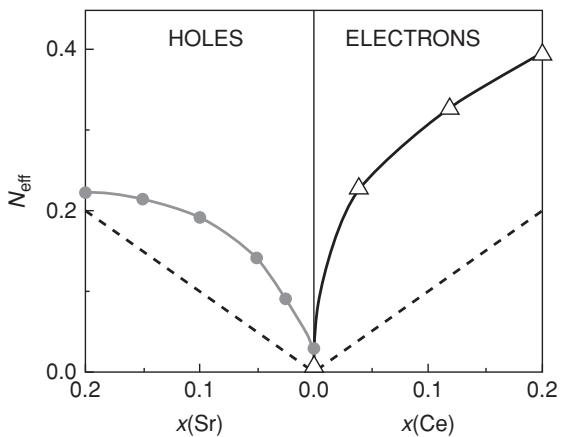
\includegraphics[width=0.55\textwidth]{figs/ch16/fig_16.11.jpg}
\caption*{图 16.11\quad 空穴掺杂（YBCO）与电子掺杂（$\mathrm{Nd}_{2-x}\mathrm{Ce}_x\mathrm{CuO}_4$，NCCO）铜氧化物的积分光电导，反映归一化载流子密度。虚线给出掺杂半导体的预期结果。在哈伯德模型内，超出名义掺杂量的电荷密度由动力学谱权重转移产生。翻印自 Cooper 等，Phys. Rev. B 41, 11605 (1990)。}\label{fig:auto:16.11}
\end{figure}
积分到光学能隙 $\Omega\approx 1.2\,\mathrm{eV}$ 为止。这是式 (9.143) 中 f 求和规则（f-sum rule）的一种形式。这里 $\sigma(\omega)$ 是光电导，$V_{\mathrm{cell}}$ 是每个化学式单胞的体积，$m$ 是自由电子质量，$e$ 是电子电荷。在没有掺杂、不形成金属态时，$N_{\mathrm{eff}}=0$。从图 16.11 可以明显看到，归一化载流子密度超过了把模型当作掺杂半导体所得的载流子密度（虚线）。在所有掺杂量下，对 $N_{\mathrm{eff}}=x$ 的偏离都是显著的。因此，任何只考虑名义掺杂量的模型都不足以描述铜氧化物中完整的低能电荷动力学。

\begin{figure}[H]\centering
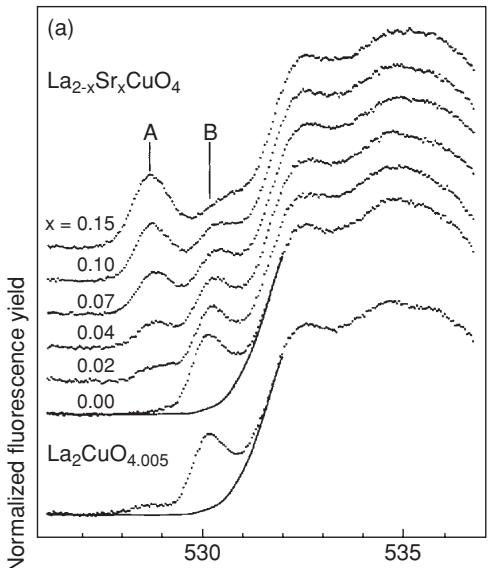
\includegraphics[width=0.5\textwidth]{figs/ch16/fig_16.12.jpg}

\vspace{0.5em}
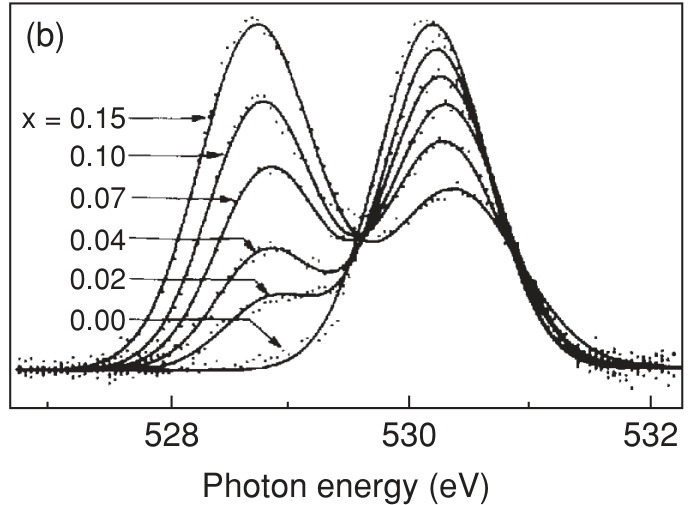
\includegraphics[width=0.6\textwidth]{figs/ch16/fig_16.12_b.jpg}
\caption*{图 16.12\quad $\mathrm{La}_{2-x}\mathrm{Sr}_x\mathrm{CuO}_{4+\delta}$ 氧 K 边的归一化荧光产额（[C1991]）。(a) 在未掺杂样品中，唯一的吸收出现在 530 eV 处，以 B 标记。掺杂后，B 处的强度转移到位于 528 eV 的 A 特征上。(b) 扣除背景后对 A、B 处吸收特征的高斯拟合。翻印自 Chen 等，Phys. Rev. Lett. 66, 104 (1991)。}\label{fig:auto:16.12}
\end{figure}
这一结果意义重大，因为它告诉我们：低能电荷自由度的数目超过裸掺杂量。因此，在强关联的语境下，最好考虑一个重正化的掺杂量 $x'\equiv x+\alpha$。本章的一个目的就是提出确定 $\alpha$ 的方法。本质上，在化学势所处的能带中，存在的并不只是裸电子。这看起来也许古怪，但事实上是真的，而且是强关联的普遍性以及谱的高、低能部分之间随之发生的混合的一部分。减去谱权重转移，得到的就是虚线（半导体）结果；然而，去掉谱权重转移同时也就去掉了强关联。最后一个值得一提的特征是 $N_{\mathrm{eff}}$ 在 $x=0$ 处的非零截距。这表明，即使在半填充，那些把莫特能隙以下的谱密度填补起来的激发仍有残余存在。这为我们理解图 16.11 中电荷计数超过虚线的起源提供了线索。

尽管光电导可用于提取有效载流子数，它终究是一个两粒子探针。因此，如果铜氧化物中载流子密度确实超过 $x$，那么从单粒子探针直接看到这一点会更有说服力。这确实可以做到。为此，我们分析图 16.12 所示的 $\mathrm{La}_{2-x}\mathrm{Sr}_x\mathrm{CuO}_4$（LSCO）的氧 $1s$ X 射线吸收实验（[C1991]）。在这类实验中，一个电子从芯态 $1s$ 被激发到一个未占据能级。实验可观测量是电子弛豫回到价态时荧光产额随能量的变化。图 16.12 的实验表明，$x=0$ 时所有可用的态都位于 530 eV 处。随掺杂增加，高能峰的强度减小，并转移到 528 eV 处的态。事实上，实验上（[C1991]）较低的峰按快于 $2x$ 的速率增长，而较高的峰按快于 $1-x$ 的速率减小，$x$ 为空穴数目。在 $\mathrm{La}_{2-x}\mathrm{Sr}_x\mathrm{CuO}_4$ 中，掺杂量 $x$ 可以毫不含糊地确定，因为每个 Sr 原子产生一个空穴。这两个峰之间的间隔就是母体绝缘材料的光学能隙。

实验中看到的谱权重的重新分布可以在哈伯德模型内得到解释。由于实验探测的是向可用的低能态的荧光产额，相应的理论量是每格点低能单粒子添加态的数目，
\begin{equation*}
L=\int_{\mu}^{\Lambda}N(\omega)\,\mathrm{d}\omega,\tag{16.117}
\end{equation*}
它定义为从化学势 $\mu$ 到截断能量尺度 $\Lambda$ 的单粒子态密度（$N(\omega)$）的积分，$\Lambda$ 划定了红外（IR）与紫外（UV）尺度的分界。费米液体中不存在上能带，$\Lambda$ 可以延伸到无穷大；而在半导体中，$\Lambda$ 只应延伸到价带顶，以计入添加空穴时可用的态。为标定这个量，我们把它与电子能够添加到掺杂剂所产生的空态上的方式数目相比较。记这个量为 $n_{\mathrm{h}}$。先考虑费米液体或无相互作用体系的情形。如图 16.2 所示，价带的总权重为 2，即每格点两个态。价带积分到化学势的权重决定填充。因此，决定 $L$ 的谱的未占据部分为 $L=2-n$。电子可以添加到空格点上的方式数目同样是 $n_{\mathrm{h}}=2-n$（见图 13.2）。于是，每电子每自旋的低能态数恒等于 1。这个结果赖以成立的关键事实是：价带总权重是一个与电子密度无关的常数。

现在考虑莫特绝缘体。在原子极限，我们已经确立（例如见式 (16.32)）：下能带的权重为 $1+x$。由于恰好有 $1-x$ 个被填充的态，$L=2x$ 在原子极限是严格的。也就是说，如图 16.4 所示，每个空穴留下一个可以被自旋向上或自旋向下电子占据的空格点。因此，基于哈伯德模型的原子极限，我们确实预期 LSCO 中 528 eV 处的荧光产额按正比于 $x$ 增长，同时在 530 eV——上哈伯德带所在的位置——有等效的减小。然而，从图 16.13 可以清楚看到，荧光产额的增长快于 $2x$。有限 $t/U$ 的哈伯德模型复现了这一结果。

\begin{figure}[H]\centering
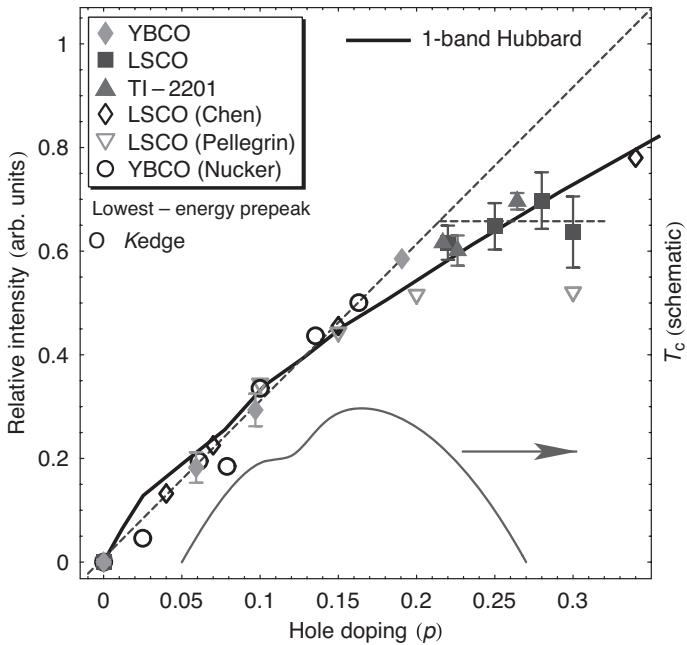
\includegraphics[width=0.62\textwidth]{figs/ch16/fig_16.13.jpg}
\caption*{图 16.13\quad 若干铜氧化物中最低能量氧 K 边前峰随掺杂变化的汇编。实直线是 A.~Liebsch（[L2010]）计算的哈伯德模型低能谱。由于实验数据的单位是任意的，用一个常数标度因子把 Liebsch 的数据点缩放后叠合到实验数据上。超导穹顶供参照。翻印自 Phillips 与 Jarrell，Phys. Rev. Lett. 105, 199701 (2010)。}\label{fig:auto:16.13}
\end{figure}

我们感兴趣的量 $L$ 可以从下能带的总权重
\begin{equation*}
m_{\mathrm{LHB}}=\frac{1}{N}\sum_{i}\big\langle\bigl\{c_{i\sigma;0},c_{i\sigma;0}^{\dagger}\bigr\}\big\rangle,\tag{16.118}
\end{equation*}
中简单地减去名义占据权重 $1-x$ 而得到。这里“名义”指的是由静态自由度确立的掺杂量，而不包括因动力学（$t/U$）效应进入的部分。这种混合意味着掺杂量本身被修改了，如图 16.11 所示。从投影到最低能量扇区的电子算符方程，即式 (16.110)，我们暂且把表达式简化为
\begin{equation*}
m_{\mathrm{LHB}}^{0}=\frac{1}{N}\sum_{i}\Big(\bigl\langle\bigl\{\tilde{\xi}_{i\sigma},\tilde{\xi}_{i\sigma}^{\dagger}\bigr\}\bigr\rangle+\Bigl\langle\frac{1}{U}\bigl(\bigl\{\tilde{\xi}_{i\sigma}^{\dagger},[\tilde{T}_{1},\tilde{\eta}_{i\sigma}]\bigr\}+\mathrm{h.c.}\bigr)\Bigr\rangle+\cdots\Big).\tag{16.119}
\end{equation*}
利用恒等式
\begin{equation*}
\tilde{\xi}_{i\sigma}\tilde{\eta}_{i\sigma}=\tilde{\xi}_{i\sigma}\tilde{\eta}_{i\sigma}^{\dagger}=0\tag{16.120}
\end{equation*}
以及基态性质 $\tilde{\eta}_{i\sigma}|G\rangle=0$，我们得到
\begin{equation*}
\big\langle\bigl\{\tilde{\xi}_{i\sigma}^{\dagger},[\tilde{T}_{1},\tilde{\eta}_{i\sigma}]\bigr\}\big\rangle=-\langle\tilde{\eta}_{i\sigma}\tilde{T}_{1}\tilde{\xi}_{i\sigma}^{\dagger}\rangle.\tag{16.121}
\end{equation*}
反复使用对易子
\begin{equation*}
\big[\tilde{n}_{i\bar{\sigma}},f_{j\sigma'}^{\dagger}\big]=\delta_{ij}\delta_{\bar{\sigma}\sigma'}f_{j\sigma'}^{\dagger},\tag{16.122}
\end{equation*}
可以把这个矩约化为两项之和：
\begin{align*}
-\langle\tilde{\eta}_{i\sigma}\tilde{T}_{1}\tilde{\xi}_{i\sigma}^{\dagger}\rangle
&=t\sum_{j,\delta,\sigma'}\big\langle f_{i\sigma}^{\dagger}\tilde{n}_{i\bar{\sigma}}\tilde{n}_{j\bar{\sigma}'}f_{j\sigma'}^{\dagger}f_{j+\delta\sigma'}(1-\tilde{n}_{j+\delta\bar{\sigma}'})(1-\tilde{n}_{i\bar{\sigma}})f_{i\sigma}^{\dagger}\big\rangle\\
&=t\sum_{j,\delta,\sigma'}\delta_{ij}\delta_{\bar{\sigma}\sigma'}\big\langle f_{i\sigma}^{\dagger}\tilde{n}_{j\bar{\sigma}'}f_{j\sigma'}^{\dagger}f_{j+\delta\sigma'}(1-\tilde{n}_{j+\delta\bar{\sigma}'})(1-\tilde{n}_{i\bar{\sigma}})f_{i\sigma}^{\dagger}\big\rangle\\
&\quad+t\sum_{j,\delta,\sigma'}\big\langle f_{i\sigma}^{\dagger}\tilde{n}_{j\bar{\sigma}'}f_{j\sigma'}^{\dagger}\tilde{n}_{i\bar{\sigma}}f_{j+\delta\sigma'}(1-\tilde{n}_{j+\delta\bar{\sigma}'})(1-\tilde{n}_{i\bar{\sigma}})f_{i\sigma}^{\dagger}\big\rangle\\
&=t\sum_{\delta}\big\langle f_{i\sigma}\tilde{n}_{i\sigma}f_{i\bar{\sigma}}^{\dagger}f_{i+\delta\bar{\sigma}}(1-\tilde{n}_{i+\delta\sigma})(1-\tilde{n}_{i\bar{\sigma}})f_{i\sigma}^{\dagger}\big\rangle\\
&\quad+t\sum_{j,\delta,\sigma'}\big\langle f_{i\sigma}^{\dagger}\tilde{n}_{j\bar{\sigma}'}f_{j\sigma'}^{\dagger}\tilde{n}_{i\bar{\sigma}}f_{j+\delta\sigma'}(1-\tilde{n}_{j+\delta\bar{\sigma}'})(1-\tilde{n}_{i\bar{\sigma}})f_{i\sigma}^{\dagger}\big\rangle,\tag{16.123}
\end{align*}
类似地使用式 (16.122) 中的对易子以及关系
\begin{equation*}
(1-\tilde{n}_{i\sigma})(1-\tilde{n}_{i\bar{\sigma}})f_{i\sigma}^{\dagger}=(1-\tilde{n}_{i\bar{\sigma}})(1-\tilde{n}_{i\sigma})f_{i\sigma}^{\dagger}=0\tag{16.124}
\end{equation*}
和
\begin{equation*}
\tilde{n}_{i\bar{\sigma}}(1-\tilde{n}_{j+\delta\bar{\sigma}'})(1-\tilde{n}_{i\bar{\sigma}})=(1-\tilde{n}_{j+\delta\bar{\sigma}'})\tilde{n}_{i\bar{\sigma}}(1-\tilde{n}_{i\bar{\sigma}})=0\tag{16.125}
\end{equation*}
可以证明，式 (16.123) 中的第二项
\begin{align*}
&\sum_{j,\delta,\sigma'}\big\langle f_{i\sigma}^{\dagger}\tilde{n}_{j\bar{\sigma}'}f_{j\sigma'}^{\dagger}\tilde{n}_{i\bar{\sigma}}f_{j+\delta\sigma'}(1-\tilde{n}_{j+\delta\bar{\sigma}'})(1-\tilde{n}_{i\bar{\sigma}})f_{i\sigma}^{\dagger}\big\rangle\\
&\quad=-t\sum_{j,\delta,\sigma'}\delta_{i,j+\delta}\delta_{\bar{\sigma}\sigma'}\big\langle f_{i\sigma}^{\dagger}\tilde{n}_{j\bar{\sigma}'}f_{j\sigma'}^{\dagger}f_{j+\delta\sigma'}(1-\tilde{n}_{j+\delta\bar{\sigma}'})(1-\tilde{n}_{i\bar{\sigma}})f_{i\sigma}^{\dagger}\big\rangle\\
&\qquad+t\sum_{j,\delta,\sigma'}\big\langle f_{i\sigma}^{\dagger}\tilde{n}_{j\bar{\sigma}'}f_{j\sigma'}^{\dagger}f_{j+\delta\sigma'}\tilde{n}_{i\bar{\sigma}}(1-\tilde{n}_{j+\delta\bar{\sigma}'})(1-\tilde{n}_{i\bar{\sigma}})f_{i\sigma}^{\dagger}\big\rangle\\
&\quad=-t\sum_{\delta}\big\langle f_{i\sigma}^{\dagger}\tilde{n}_{i-\delta\sigma}f_{i-\delta\bar{\sigma}}^{\dagger}f_{i\bar{\sigma}}(1-\tilde{n}_{i\sigma})(1-\tilde{n}_{i\bar{\sigma}})f_{i\sigma}^{\dagger}\big\rangle\\
&\qquad+t\sum_{j,\delta,\sigma'}\big\langle f_{i\sigma}^{\dagger}\tilde{n}_{j\bar{\sigma}'}f_{j\sigma'}^{\dagger}f_{j+\delta\sigma'}\tilde{n}_{i\bar{\sigma}}(1-\tilde{n}_{j+\delta\bar{\sigma}'})(1-\tilde{n}_{i\bar{\sigma}})f_{i\sigma}^{\dagger}\big\rangle=0\tag{16.126}
\end{align*}
恒为零。我们已接近完成。剩余项中还有几个因子可以用恒等式
\begin{align*}
f_{i\sigma}\tilde{n}_{i\sigma}&=f_{i\sigma},\\
f_{i\bar{\sigma}}^{\dagger}(1-\tilde{n}_{i\bar{\sigma}})&=f_{i\bar{\sigma}}^{\dagger}.\tag{16.127}
\end{align*}
加以简化。于是
\begin{align*}
-\langle\tilde{\eta}_{i\sigma}\tilde{T}_{1}\tilde{\xi}_{i\sigma}^{\dagger}\rangle
&=t\sum_{\delta}\big\langle f_{i\sigma}\tilde{n}_{i\sigma}f_{i\bar{\sigma}}^{\dagger}f_{i+\delta\bar{\sigma}}(1-\tilde{n}_{i+\delta\sigma})(1-\tilde{n}_{i\bar{\sigma}})f_{i\sigma}^{\dagger}\big\rangle\\
&=t\sum_{\delta}\big\langle f_{i\sigma}\tilde{n}_{i\sigma}f_{i\sigma}^{\dagger}f_{i\bar{\sigma}}^{\dagger}(1-\tilde{n}_{i\bar{\sigma}})f_{i+\delta\bar{\sigma}}(1-\tilde{n}_{i+\delta\sigma})\big\rangle\\
&=t\sum_{\delta}\big\langle f_{i\sigma}f_{i\sigma}^{\dagger}f_{i\bar{\sigma}}^{\dagger}f_{i+\delta\bar{\sigma}}(1-\tilde{n}_{i+\delta\sigma})\big\rangle\\
&=t\sum_{\delta}\Big\langle(1-\tilde{n}_{i\sigma})f_{i\bar{\sigma}}^{\dagger}f_{i+\delta\bar{\sigma}}(1-\tilde{n}_{i+\delta\sigma})\Big\rangle.\tag{16.128}
\end{align*}
由于平均是对一个不存在 $f_{i\sigma}$ 费米子双占据的基态作的，带密度因子 $\tilde{n}_{i\sigma}$ 的项全部消失，于是下能带的总权重
\begin{equation*}
m_{\mathrm{LHB}}=1+x+\frac{2t}{U}\frac{1}{N}\sum_{i\delta\sigma}\big\langle f_{i\bar{\sigma}}^{\dagger}f_{i+\delta\bar{\sigma}}\big\rangle+\cdots=1+x+\alpha(t/U,x)>1+x,\tag{16.129}
\end{equation*}
带有显式的 $t/U$ 修正，其第一项正比于下能带中因双占据的动力学产生而出现的空格点的动能。我们用 $\alpha$ 表示所有 $t/U$ 修正，它是谱权重动力学转移的量度。这个公式的一个版本最初由 Harris 与 Lange（[HL1967]）于 1967 年导出，并在文献 [E1994] 中用正确的算符重新导出。值得注意的是，出现在这个表达式中的算符是变换后的费米子，而不是裸费米子。当然，可以只用裸费米子表示下能带的谱权重，但表达式相当繁琐（[E1994]）。同样值得注意的是，无论微扰论的阶数如何，$\alpha$ 都严格为正（[HL1967; E1994; MES1993]）。道理很简单：下能带中的动力学只能以产生双占据格点为代价。这必然使上能带的强度减小（见图 16.14），因为现在产生双占据的方式变少了。为保持谱权重守恒，下能带的强度必须增加同等的量。本质上，动力学谱权重转移之所以存在，是因为算符 $\xi_{i\sigma}$ 与 $\eta_{i\sigma}$ 在任何能量尺度上都不能独立传播。若把下能带谱的占据部分赋以守恒电荷 $1-x$ 的权重，则下能带谱的未占据部分携带权重 $2x+\alpha>2x$。然而，没有必要固守对谱的这种划分，因为一旦一个能带的权重超过该能带中电子态的总数，即 $1+x+\alpha>1+x$，电子究竟在做什么就无关紧要了。我们从图 16.11 知道，有效掺杂量超过 $x$。图 16.14(b) 中对谱权重的划分（[CHP2010]）反映了载流子的动力学产生。采用这种划分，LHB 中每自旋的谱未占据部分恰好就是有效掺杂量 $x'$。也就是说，对谱的这种划分恢复了原子极限下的半刚性能带图像，如图 16.4 那样。图 16.13 把 $L$ 的实验值与哈伯德模型上最先进的计算（实线）作了比较。解读实验值时需要提醒一句。由于强度是用任意单位表示的，$y$ 轴并不真正对应能带未占据部分的实际谱密度。注意虚线的斜率为 3。因此，不应把这条直虚线理解为氧 K 边谱按 $2x$ 增长的量度。为了在哈伯德模型的结果与实验之间进行比较，哈伯德数据经过了适当的标度。引人注目的是，在所研究的掺杂范围内，实线与实验值在定量上符合得相当好。在空穴掺杂量 $p\approx 0.18$ 附近，数据与虚线（它从原点出发）有明显偏离。哈伯德模型同样复现了这一偏离，它标志着超过某个临界掺杂值之后，动力学修正急剧减小。原因很简单：动力学修正必须在 $x=1$ 处消失，因此它不可能单调增加。

\begin{figure}[H]\centering
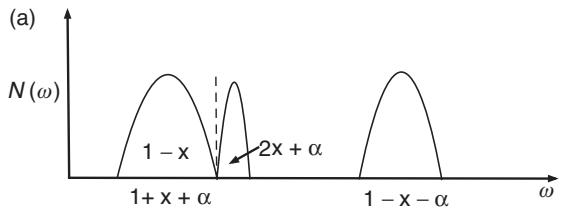
\includegraphics[width=0.62\textwidth]{figs/ch16/fig_16.14_a.jpg}

\vspace{0.5em}
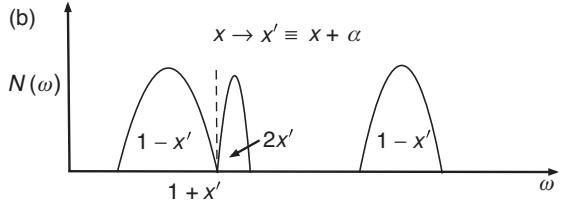
\includegraphics[width=0.62\textwidth]{figs/ch16/fig_16.14_b.jpg}
\caption*{图 16.14\quad 哈伯德模型中单粒子态密度随空穴掺杂量 $x$ 的变化。$\alpha$ 表示式 (16.129) 所刻画的谱权重的动力学即 $t/U$ 修正。(a) 下能带谱权重的传统划分，其中下能带被占据的部分就是守恒电荷。(b) 计及图 16.11 中所见掺杂量重正化的谱权重划分。}\label{fig:auto:16.14}
\end{figure}

$d=1$ 的哈伯德模型为计算 $\alpha$ 提供了一个基准。在这种情形下，$\alpha$ 可以用贝特拟设（Bethe ansatz）（[LW1968]）方法结合动力学矩阵重正化群（[K2010]）来计算进入谱函数的动力学关联函数，从而基本上精确地确定。图 16.15 给出了下哈伯德带中谱密度在化学势以下（方块）和以上的积分权重的结果。图 16.15 中的星号代表谱的占据部分，$1-x$。每自旋其余的谱权重（圆圈，$U=4t$；方块，$U=8t$）给出 $L$（按照图 16.14(a) 计算）的量度。显然，两者都超过虚线，正如式 (16.129) 的微扰展开所预期，并与图 16.13 所示的二维计算一致。一般地，对任何有限维晶格，动力学谱权重转移都是不可避免的。

\begin{figure}[H]\centering
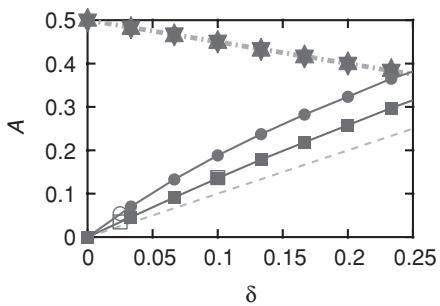
\includegraphics[width=0.5\textwidth]{figs/ch16/fig_16.15.jpg}
\caption*{图 16.15\quad $d=1$ 哈伯德模型中下能带每自旋的积分谱权重。星号代表下能带的占据部分。实心方块与圆圈分别对应 $U=8t$ 和 $U=4t$ 时的粒子添加部分（恰在化学势之上）。虚线的斜率为 1。翻印自 Kohno，Phys. Rev. Lett. 105, 106402 (2010)。}\label{fig:auto:16.15}
\end{figure}

动力学谱权重转移之所以重要，是因为它产生了一种全新的定性效应。它是“多”则全然不同（``more'' being totally different）的一个例子（[A1972]）。费米液体中，一个能带的强度等于该能带所能容纳的电子数。而在存在动力学谱权重转移时，下能带和能带未占据部分的强度都超过这些态在低能下所能容纳的电子数，与费米液体形成鲜明对照。能装进下能带的电子数只由格点数目决定，而不依赖于诸如 $t$ 和 $U$ 这样的体系参数，因此它固定在 $1+x$。同样，下能带谱的未占据部分只能以 $2x$ 种方式被电子占据。然而，至少有 $2x+\alpha$ 个态可供粒子添加。结果，对下能带物理的任何描述都无法仅凭数电子来穷尽。本质上，如果一个能带的总谱权重超过电子计数——此处即 $1+x+\alpha>1+x$——那么电子究竟在做什么就无关紧要。这凸显了强耦合的关键要素：传播自由度与原始紫外完备理论中的基本构件毫无相似之处。例如考虑 $L$。$L$ 量度的是向 下能带添加一个粒子的总谱密度。若它按每自旋超过 $x$，则添加一个粒子的方式总数超过向下能带添加一个\emph{电子}的方式数。因此，$L/2>x$ 意味着下能带中有些粒子添加态对添加一个电子是有能隙的。也就是说，下能带中有些态与添加一个电子正交。产生这种正交性的态是与上能带混合的态。因此，正是上能带的单纯存在在下能带中产生了这段有能隙的谱。既然上能带完全源于强关联，混入下能带的这些额外的态在弱相互作用体系中没有对应物，费米液体理论便告失效。由此，动力学谱权重转移为下能带中有效费米液体描述的失效提供了一个具体机制。虽然安德森（[A1997]）早先已假定上哈伯德带会在低能下导致对电子添加的正交性，但他并未明确把动力学谱权重转移指认为这种正交性的具体机制。事实上，他近期的工作（[A2006]）专注于严格从 $U=\infty$ 极限——动力学修正在此消失——提取这种正交性。

\begin{figure}[H]\centering
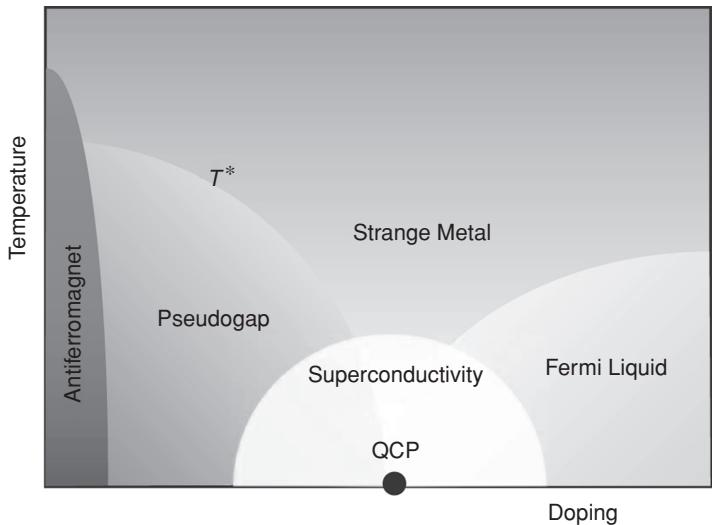
\includegraphics[width=0.7\textwidth]{figs/ch16/fig_16.16.jpg}
\caption*{图 16.16\quad 掺入铜氧面的空穴浓度的示意相图。赝能隙与奇异金属分别以态密度的亏耗和 $T$ 线性电阻率为特征。赝能隙终止于一个零温临界点，即量子临界点（QCP）。右侧是弱耦合描述成立的费米液体区。}\label{fig:auto:16.16}
\end{figure}

对电子添加的正交性是铜氧化物正常态的核心问题。图 16.16 给出了铜氧化物的示意相图，其中突出标出了掺杂莫特绝缘体后出现的关键角色。赝能隙与奇异金属是正常态中我们关心的两个相。在赝能隙区，存在能隙但没有超导。与费米液体不同，奇异金属表现出 $T$ 线性电阻率。的确，正如相图所提示的，奇异金属与赝能隙紧密相连。实验上，$T^{*}$ 线由输运测量确定为 $T$ 线性电阻率出现的最低温度（[KLR2001; AKS2004]）。由于超导态具有 $d_{x^{2}-y^{2}}$ 对称性（[H1995]），布里渊区对角线代表节点方向。图 16.17 绘出的是对铜氧化物中沿布里渊区对角线的电子格林传播子的极点
\begin{equation*}
G(\omega,\mathbf{q})=\frac{Z}{\omega-\epsilon_{\mathrm{F}}}\tag{16.130}
\end{equation*}
强度的高精度测量。关于式 (16.130) 的解读需要说明几句。即使电子传播子带有如式 (16.58) 那样的自能，像式 (16.130) 这样的表达式仍然成立。只需围绕费米能展开自能，
\begin{equation*}
\Sigma(\omega,\mathbf{k})=\Sigma_{0}+(\omega-\epsilon_{\mathrm{F}})\frac{\partial\Sigma^{\mathrm{R}}(\omega,\mathbf{k})}{\partial\omega}\Big|_{\omega=\epsilon_{\mathrm{F}}}+\cdots,\tag{16.131}
\end{equation*}

\begin{figure}[H]\centering
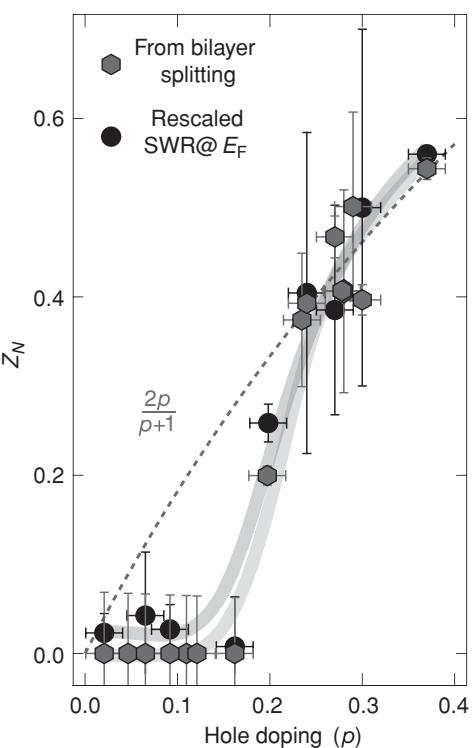
\includegraphics[width=0.45\textwidth]{figs/ch16/fig_16.17.jpg}
\caption*{图 16.17\quad YBCO 中由角分辨光电子能谱测得的准粒子权重。准粒子权重的消失表明铜氧化物的正常态是非费米液体。翻印自 Fournier 等，Nat. Phys. 6, 905 (2010)。}\label{fig:auto:16.17}
\end{figure}
只保留一阶导数项，我们把准粒子权重表示为
\begin{equation*}
Z=(1-\partial\Sigma^{\mathrm{R}}/\partial\omega)^{-1}.\tag{16.132}
\end{equation*}
费米液体中，每个掺杂剂都在化学势上方产生一个准粒子激发，因此准粒子权重预期按 $x$ 标度。铜氧化物中情形并非如此。令人注目的是，准粒子权重（[F2010]）在掺杂量 0.15 附近消失，表明超导电性由之涌现的底层状态是一个非费米液体，其中电子并不是传播自由度。传播模式究竟是什么，正是铜氧化物的核心问题。图 16.17 用来比较准粒子权重的理论（[A2004]）给出 $Z\propto 2x/(1+x)$。这个表达式只应在 $x=0$ 处消失。该公式的来历不过是把准粒子权重的费米液体形式应用于静态部分，即严格从下能带谱权重的态计数得出的那部分。按照费米液体理论，准粒子权重应按谱的未占据部分、并以能带的总强度加权来标度。既然有 $2x$ 个粒子添加态，而能带的总权重为 $1+x$，结果 $Z=2x/(1+x)$ 是自然的。然而，数据（见图 16.17）表明该公式失效。

如上所述，动力学谱权重转移为费米液体理论的失效、从而为 $Z$ 的消失提供了一个自然机制。归根到底，如果动力学谱权重转移是费米液体理论失效的机制，那么这种物理在超导态中应当仍然存在，因为它对有序化并不敏感。事实确实如此。为引导这里的讨论，我们关注 f 求和规则
\begin{equation*}
A=\frac{\pi n_{e}e^{2}}{m}=\int_{0}^{\infty}\sigma(\omega)\,\mathrm{d}\omega.\tag{16.133}
\end{equation*}
为理解高 $T_{\mathrm{c}}$ 超导体中的谱变化，把 $A$ 分解为低能分量
\begin{equation*}
A_{\mathrm{l}}=\int_{0^{+}}^{\Omega}\sigma(\omega)\,\mathrm{d}\omega,\tag{16.134}
\end{equation*}
和高能部分
\begin{equation*}
A_{\mathrm{h}}=\int_{\Omega}^{\infty}\sigma(\omega)\,\mathrm{d}\omega.\tag{16.135}
\end{equation*}
是有帮助的。截断 $\Omega$ 的选取使得 $A_{\mathrm{h}}$ 严格包含与带间跃迁相联系的谱权重。通常取 $\Omega/(2\pi c)=10\,000\,\mathrm{cm}^{-1}$ 便足以界定 $\sigma(\omega)$ 的极小值，该极小值标志带内跃迁与带间跃迁的分界，本质上就是下、上哈伯德带之间的截断。回忆式 (9.136)，电导率有如下形式的虚部
\begin{equation*}
\mathrm{Im}\,\sigma(\omega)=\frac{n_{e}e^{2}/m}{\omega}.\tag{16.136}
\end{equation*}
只有在超导体中，这一贡献才不为零。由克拉默斯—克勒尼希（Kramers--Kronig）关系
\begin{equation*}
\mathrm{Im}\,\sigma(\omega)=\frac{1}{\pi}\,\mathrm{P}\int_{-\infty}^{\infty}\frac{\mathrm{d}\omega'\,\mathrm{Re}\,\sigma(\omega')}{\omega'-\omega},\tag{16.137}
\end{equation*}
与式 (16.136) 相容的电导率实部为 $\mathrm{Re}\,\sigma(\omega)=A\delta(\omega)$。在超导体中，$\hbar\omega<2\Delta$（$\Delta$ 为超导能隙）范围内被移走的谱权重转移到零频率处的 $\delta$ 函数上。$\delta$ 函数中的权重必定等于凝聚到超导态时被移走的谱权重。这一效应由 Ferrell--Glover--Tinkham（[T2004]）求和规则描述：
\begin{equation*}
D=A_{\mathrm{l}}^{\mathrm{n}}-A_{\mathrm{l}}^{\mathrm{s}}+A_{\mathrm{h}}^{\mathrm{n}}-A_{\mathrm{h}}^{\mathrm{s}},\tag{16.138}
\end{equation*}
其中上标 n 与 s 分别指正常态与超导态。BCS 超导体的特征是高、低能量尺度之间有清晰的分界，$D$ 中没有来自 $A_{\mathrm{h}}$ 的贡献。通常，只需积分到不超过 $10\Delta$ 便能恢复 $D$。然而，在高 $T_{\mathrm{c}}$ 超导体中，椭偏实验（[RG2001]）观察到介电函数在转变到超导态时的变化延伸到 $100\Delta$，这对铜氧化物而言暗示了另一种情形。

\begin{figure}[H]\centering
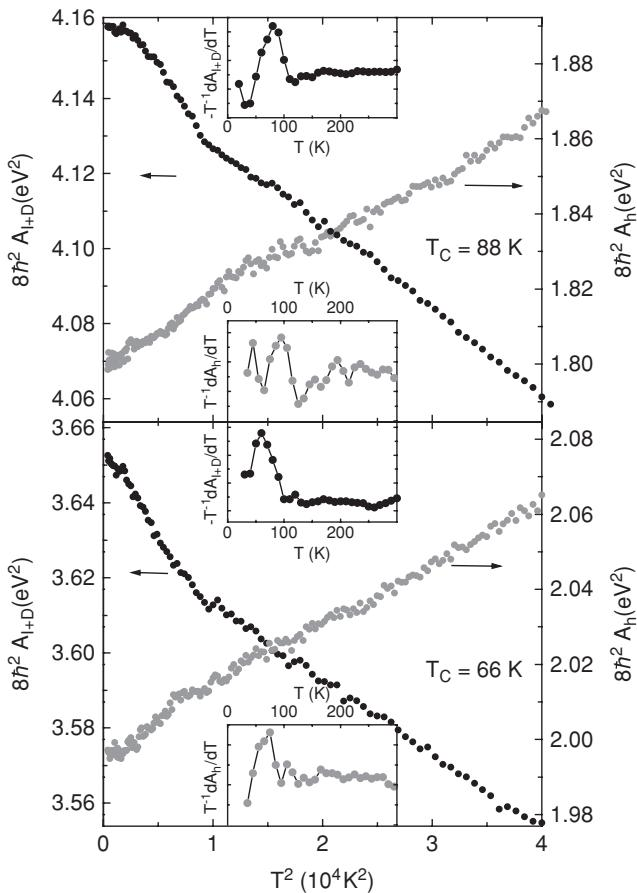
\includegraphics[width=0.48\textwidth]{figs/ch16/fig_16.18.jpg}
\caption*{图 16.18\quad 最佳掺杂（上）与欠掺杂（下）的 $\mathrm{Bi}_2\mathrm{Sr}_2\mathrm{CaCu}_2\mathrm{O}_{8-\delta}$ 的低频谱权重 $A_{\mathrm{l}+D}(T)$ 与高频谱权重 $A_{\mathrm{h}}(T)$ 随温度的变化。插图给出这两个量的导数乘以 $T^{-1}$。翻印自 Molegraaf 等，Science 295, 5563 (2002)。}\label{fig:auto:16.18}
\end{figure}

对 BSCCO（译注：原文为 BSCO）（[M2002]），无论最佳掺杂还是欠掺杂样品，当温度降到 $T_{\mathrm{c}}$ 以下时，$A_{\mathrm{h}}$ 表现出加速的减小，同时 $A_{\mathrm{l}}$ 补偿性地增加，如图 16.18 所示。这表明，正是高能区谱权重的损失驱动了超导态。这些数据还与其他光学测量一致——后者表明，把光电导积分到 2 eV 便能恢复超导态中 $\delta$ 函数的全部权重（[SL2003]）；也与数值计算一致——后者表明，哈伯德模型中随频率变化的配对相互作用包含一个完全来自上哈伯德带的非推迟部分（[MPS2008]）。这种从可见光到红外波段的“变色”意味着，铜氧化物中的超导电性与金属中的存在本质差别。也就是说，在铜氧化物中，超导电性并非只关乎费米面上的低能物理。正确的理论应当精确解释，高能处（距化学势 2 eV）的谱权重损失如何导致超流密度的增长。

\section{尾声：$1=2-1$}

正如我们所见，铜氧化物体现了固体物理学三大支柱的失效：(1) 金属的能带论，(2) 费米液体理论，(3) 超导电性的 BCS 理论。这一概念三联体的核心是刚性带概念的缺席。如本章开头所述，UHB 与 LHB 并非传统意义上的能带。尽管如此，我们可以遵循上文概述的微扰流程，依据在原子极限中获得的直觉对谱进行划分。式 (16.129) 意味着，下能带的总强度超过 $1+x$，即下能带中电子态的总数。动力学修正 $\alpha$ 在实验上可以直接观测：既可以在 X 射线 K 边实验（[C1991]）中，也可以在光学测量（[C1990]）中，这些测量表明有效掺杂量超过裸空穴计数 $x$。一个能带的强度怎么可能超过该能带中电子态的数目？能带中显然必定还有别的东西，而且它必定携带电荷 $e$，因为强度所计数的正是电荷为 $e$ 的激发的数目。这些额外的电荷 $e$ 激发是什么？我们有两种选择：要么把电子的自旋与电荷拆开，要么选择复合激发。把自旋与电荷拆开并不能解决额外强度的问题，因为这不可能给出大于 $1+x$ 的强度。唯一的选择是复合激发。本节标题中的那个方程给出了答案：$1=2-1$。一个电荷为 $2e$ 的实体与电荷为 $-e$ 的空穴相束缚，正合所需。结果是一个电荷为 $e$ 的复合激发。可以想象更复杂的方案，但 $1=2-1$ 是最简单的。而且，这在物理上是合理的。动力学谱权重转移所涉及的，恰恰就是莫特（[M1949]）以及其他人（[KHF1982; K1964; C1979]）论证过必须束缚在一起以传递莫特能隙的那类激发（见图 16.7）。有限掺杂时，这类激发依然存在。它们代表双占据格点与空格点上的空穴之间的束缚态，从而为 $1=2-1$ 提供了一条物理途径。本质上，低能下的双占据代表一种集体激发，它源于下、上能带刚性的缺失。这种激发可以在一个场论中具体实现（[LPC2007; P2010]）：对上能带引入一个约束，使得约束保持时上能带是刚性的；一旦约束放宽，一个电荷为 $2e$ 的玻色场就会作为低能集体激发出现，正如电子气问题中，一旦放宽对扩展希尔伯特空间的约束，等离激元便应运而生。事实上，严格积掉上哈伯德带所用的技巧（[LPC2007; P2010]）（超出了本书的范围）与第 9 章在等离激元的语境中引入的集体场论方法完全相同。一个电荷为 $2e$ 的集体场（显然是玻色性的，且不同于诸如库珀对之类的任何东西。库珀对由基本激发构成；而电荷 $2e$ 玻色子源于动力学，因而并非如此）在低能出现，并与空穴相束缚，这正是强耦合物理的典型表现。具体地说，新的激发（通常是复合物）作为低能的传播自由度出现，它们在紫外完备理论中没有对应物。这类激发也解决了图 16.17 中的正交性问题。由于它们拥有内部自由度，它们与裸电子正交，从而为图 16.17 中 $Z\to 0$ 的问题提供了一种解决之道。于是，简单的方程 $1=2-1$ 包含了动力学谱权重转移的精髓。图 16.18 的实验表明，负责动力学谱权重转移的这类激发，在铜氧化物的超导问题中扮演着关键却未知的角色。

\section*{习题}
\addcontentsline{toc}{section}{习题}

\textbf{习题 16.1}\quad 计及最近邻相互作用的哈伯德模型具有形式
\begin{equation*}
H_{\mathrm{Hubb}}=-t\sum_{i,j,\sigma}\big(\eta_{i\sigma}^{\dagger}\eta_{j\sigma}+\xi_{i\sigma}^{\dagger}\xi_{j\sigma}+\eta_{i\sigma}^{\dagger}\xi_{j\sigma}\big)+\frac{U}{2}\sum_{i,\sigma}\eta_{i\sigma}^{\dagger}\eta_{i,\sigma}+V\sum_{i,j}n_{i}n_{j},\tag{16.139}
\end{equation*}
其中 $n_{i}=n_{i\uparrow}+n_{i\downarrow}$。证明：使该模型在式 (16.39) 之下保持不变的化学势取值为 $\mu=(U+2V)/2$。

\textbf{习题 16.2}\quad 显式证明系数为
\begin{align*}
\alpha_{n+1}&=(U-\mu)\alpha_{n}+U(-\mu)^{n},\\
\beta_{n}&=(-\mu)^{n},\tag{16.140}
\end{align*}
所用的递推关系是
\begin{equation*}
Q_{i\sigma}^{(n+1)}=\big[Q_{i\sigma}^{(n)},H_{U}\big].\tag{16.141}
\end{equation*}

\textbf{习题 16.3}\quad 导出半填充哈伯德二聚体的所有本征态和本征值。所谓半填充，我指的是两个电子占据两个格点，一个自旋向上，另一个自旋向下。对基态，你应当得到式 (16.80)。

\textbf{习题 16.4}\quad 考虑一个算符 $O$。一般地
\begin{equation*}
O=\sum_{n\in\mathbb{Z}}O_{nU}.\tag{16.142}
\end{equation*}
你的任务是用变换后的算符 $\tilde{O}$ 导出 $O_{nU}$ 的显式表达式。由一般表达式
\begin{equation*}
O=\mathrm{e}^{S}\tilde{O}\mathrm{e}^{-S}\tag{16.143}
\end{equation*}
证明
\begin{align*}
O_{nU}&=\tilde{O}_{nU}+\frac{1}{U}\big[\tilde{T}_{1},\tilde{O}_{(n-1)U}\big]-\frac{1}{U}\big[\tilde{T}_{-1},\tilde{O}_{(n+1)U}\big]\\
&\quad+\frac{1}{U^{2}}\Big(\big[\big[\tilde{T}_{1},\tilde{T}_{0}\big],\tilde{O}_{(n-1)U}\big]+\big[\big[\tilde{T}_{-1},\tilde{T}_{0}\big],\tilde{O}_{(n+1)U}\big]\\
&\quad+\frac{1}{2}\big[\tilde{T}_{1},\big[\tilde{T}_{1},\tilde{O}_{(n-2)U}\big]\big]+\frac{1}{2}\big[\tilde{T}_{-1},\big[\tilde{T}_{-1},\tilde{O}_{(n+2)U}\big]\big]\\
&\quad-\frac{1}{2}\big[\tilde{T}_{1},\big[\tilde{T}_{-1},\tilde{O}_{nU}\big]\big]-\frac{1}{2}\big[\tilde{T}_{-1},\big[\tilde{T}_{1},\tilde{O}_{nU}\big]\big]\Big).\tag{16.144}
\end{align*}

\section*{参考文献}
\addcontentsline{toc}{section}{参考文献}

\begin{itemize}[leftmargin=2em,itemsep=0pt,parsep=0pt,label={}]
\item {[AZ1988]} I.~Affleck, Z.~Zou, T.~Hsu, and P.~W. Anderson, \emph{Phys. Rev. B} \textbf{38}, 745 (1988).
\item {[A1972]} This is a rephrasing of the essay title ``More is Different'' by P.~W. Anderson, \emph{Science} \textbf{177}, 393 (1972).
\item {[A1987]} P.~W. Anderson, \emph{Science} \textbf{235}, 1196 (1987).
\item {[A1997]} P.~W. Anderson, \emph{The Theory of Superconductivity in the High-$T_{c}$ Cuprates} (Princeton Series in Physics, Princeton University Press, 1997).
\item {[A2006]} P.~W. Anderson, \emph{Nat. Phys.} \textbf{2}, 626 (2006).
\item {[A2004]} P.~W. Anderson, P.~A. Lee, M.~Randeria, T.~M. Rice, N.~Trivedi, and F.~C. Zhang, \emph{J. Phys.: Cond. Matt.} \textbf{16}, R755 (2004).
\item {[AKS2004]} Y.~Ando, S.~Komiya, K.~Segawa, S.~Ono, and Y.~Kurita, \emph{Phys. Rev. Lett.} \textbf{93}, 267001 (2004).
\item {[C1979]} C.~Castellani, C.~Di Castro, D.~Feinberg, and J.~Ranninger, \emph{Phys. Rev. Lett.} \textbf{43}, 1957 (1979).
\item {[CHP2010]} S.~Chakraborty, S.~Hong, and P.~Phillips, \emph{Phys. Rev. B} \textbf{81}, 235135 (2010).
\item {[C1991]} C.~T. Chen, F.~Sette, Y.~Ma, \emph{et al.}, \emph{Phys. Rev. Lett.} \textbf{66}, 104 (1991).
\item {[C2004]} A.~L. Chernyshev, D.~Galanakis, P.~Phillips, A.~V. Rozhkov, and A.-M.~S. Tremblay, \emph{Phys. Rev. B} \textbf{70}, 235111 (2004).
\item {[C1990]} S.~L. Cooper, G.~A. Thomas, J.~Ornstein, \emph{et al.}, \emph{Phys. Rev. B} \textbf{41}, 11605 (1990).
\item {[C1993]} S.~L. Cooper, D.~Reznik, A.~Kotz, \emph{et al.}, \emph{Phys. Rev. B} \textbf{47}, 8233 (1993).
\item {[DFM1988]} E.~Dagotto, E.~Fradkin, and A.~Moreo, \emph{Phys. Rev. B} \textbf{38}, 2926 (1988).
\item {[D2003]} I.~Dzyaloshinskii, \emph{Phys. Rev. B} \textbf{68}, 085113 (2003).
\item {[E1994]} H.~Eskes, A.~M. Ole\'{s}, M.~B.~J. Meinders, and W.~Stephan, \emph{Phys. Rev. B} \textbf{50}, 17980 (1994).
\item {[F2010]} D.~Fournier, G.~Levy, Y.~Pennec, \emph{et al.}, \emph{Nat. Phys.} \textbf{6}, 905 (2010).
\item {[GKKR1996]} A.~Georges, G.~Kotliar, W.~Krauth, and M.~J. Rozenberg, \emph{Rev. Mod. Phys.} \textbf{68}, 13 (1996).
\item {[G1971]} J.~B. Goodenough, \emph{J. Solid State Chem.} \textbf{3}, 490 (1971).
\item {[H1991]} F.~D.~M. Haldane, \emph{Phys. Rev. Lett.} \textbf{67}, 937 (1991).
\item {[H1995]} D.~J. van Harlingen, \emph{Rev. Mod. Phys.} \textbf{67}, 515 (1995).
\item {[HL1967]} A.~B. Harris and R.~V. Lange, \emph{Phys. Rev.} \textbf{157}, 295 (1967).
\item {[H1974]} G.~'t Hooft, \emph{N. Phys. B} \textbf{75}, 461 (1974).
\item {[H1963]} J.~Hubbard, \emph{Proc. Roy. Soc. London, Ser. A}, \textbf{276}, 238 (1963).
\item {[J1992]} M.~Jarrell, \emph{Phys. Rev. Lett.} \textbf{69}, 168 (1992).
\item {[KHF1982]} T.~A. Kaplan, P.~Horsch, and P.~Fulde, \emph{Phys. Rev. Lett.} \textbf{49}, 889 (1982).
\item {[K1964]} W.~Kohn, \emph{Phys. Rev.} \textbf{133}, A171 (1964).
\item {[K2010]} M.~Kohno, \emph{Phys. Rev. Lett.} \textbf{105}, 106402 (2010).
\item {[KLR2001]} Z.~Konstantinovic, Z.~Z. Li, and H.~Raffy, \emph{Physica C} \textbf{351}, 1653 (2001).
\item {[L2005]} Y.~S. Lee, K.~Segawa, Z.~Q. Li, \emph{et al.}, \emph{Phys. Rev. B} \textbf{72}, 054529 (2005).
\item {[LPC2007]} R.~G. Leigh, P.~Phillips, and T.-P. Choy, \emph{Phys. Rev. Lett.} \textbf{99}, 046404 (2007).
\item {[LW1968]} E.~H. Lieb and F.~Y. Wu, \emph{Phys. Rev. Lett.} \textbf{20}, 1445 (1968).
\item {[L2010]} A.~Liebsch, \emph{Phys. Rev. B} \textbf{81}, 235133 (2010).
\item {[MPS2008]} T.~A. Maier, D.~Poilblanc, and D.~J. Scalapino, \emph{Phys. Rev. Lett.} \textbf{100}, 237001 (2008).
\item {[MES1993]} M.~B.~J. Meinders, H.~Eskes, and G.~A. Sawatzky, \emph{Phys. Rev. B} \textbf{48}, 3916 (1993).
\item {[M2002]} H.~J.~A. Molegraaf, C.~Presura, D.~van der Marel, P.~H. Kes, and M.~Li, \emph{Science} \textbf{295}, 2239 (2002).
\item {[M1949]} N.~F. Mott, \emph{Proc. Phys. Soc. A} \textbf{62}, 416 (1949).
\item {[P2010]} P.~Phillips, \emph{Rev. Mod. Phys.} \textbf{82}, 1719 (2010).
\item {[Q2008]} M.~M. Qazilbash, A.~A. Schafgans, K.~S. Burch, \emph{et al.}, \emph{Phys. Rev. B} \textbf{77}, 115121 (2008).
\item {[RLP1994]} T.~M. Rice, H.~Launois, and J.~P. Pouget, \emph{Phys. Rev. Lett.} \textbf{73}, 3042 (1994).
\item {[R2007]} A.~Rosch, \emph{Eur. Phys. J. B} \textbf{59}, 495 (2007).
\item {[RG2001]} M.~R\"{u}bhausen, A.~Gozar, M.~V. Klein, P.~Guptasarma, and D.~G. Hinks, \emph{Phys. Rev. B} \textbf{63}, 224514 (2001).
\item {[SL2003]} A.~F. Santander-Syro, R.~P.~S.~M. Lobo, N.~Bontemps, Z.~Konstantinovic, Z.~Z. Li, and H.~Raffy, \emph{Eur. Phys. Lett.} \textbf{62}, 568 (2003).
\item {[SPC2007]} T.~D. Stanescu, P.~Phillips, and T.-P. Choy, \emph{Phys. Rev. B} \textbf{75}, 104503 (2007).
\item {[S2010]} I thank M.~Sobol for suggesting presenting the Mott problem starting from this model.
\item {[T2004]} M.~Tinkham, \emph{Introduction to Superconductivity} (Dover, 2004), 2nd edition.
\item {[ZR1988]} F.~C. Zhang and T.~M. Rice, \emph{Phys. Rev. B} \textbf{37}, 3759 (1988).
\item {[ZM1975]} A.~Zylbersztejn and N.~F. Mott, \emph{Phys. Rev. B} \textbf{11}, 4383 (1975).
\end{itemize}
